\documentclass{article}

\usepackage[utf8]{inputenc}
\usepackage{graphicx}
\usepackage{listings}
\usepackage{color}
\usepackage{float}
\usepackage{multicol}

\definecolor{dkgreen}{rgb}{0,0.6,0}
\definecolor{gray}{rgb}{0.5,0.5,0.5}
\definecolor{mauve}{rgb}{0.58,0,0.82}

\lstset{frame=tb,
    language=C,
    aboveskip=3mm,
    belowskip=3mm,
    showstringspaces=false,
    columns=flexible,
    basicstyle={\small\ttfamily},
    numbers=left,
    numberstyle=\tiny\color{gray},
    keywordstyle=\color{blue},
    commentstyle=\color{dkgreen},
    stringstyle=\color{mauve},
    breaklines=true,
    breakatwhitespace=true,
    tabsize=3
}


\title{TP 4 IA: Cartes de Kohonen}
\date{\today}
\author{Djahid ABDELMOUMENE}

\begin{document}
\maketitle

\section{Exerice 1}
\subsection{Gestion des données}
\begin{itemize}
   \item
      Le structure de réseau kohonen:
      \begin{lstlisting}
      typedef struct kohonen {
         float **weight; // les poids de réseau
         float *input; // les entrées de neurones
         int sizeX, sizeY; // la topologie de réseau
         int sizeInput; // la taille de vecteur d'entrée
         int winner; // l'indice de neurone gagnant
         float (*phi)(float); // fonction de voisinage
         float (*topDist)(int, int, int, int); // fonction de distance topologique
      } KOHONEN;
      \end{lstlisting}

\end{itemize}

\subsection{Apprentissage}
\paragraph{Extension de IHM:}\\
   L'IHM pour l'exercice 2 (MODE=1) affiche les positions des villes et
les neurones avec les connections topologique entre eux, et pour le
controle, $P$ pour commencer et arrêter l'apprentissage, $S$ pour
chercher le chemin trouvé par le réseau, $R$ pour réinitialiser les
valeurs des poids aléatoirement, $Q$ pour quitter.\\
\vspace{1mm}

Pour l'execice 3 (MODE=0) affiche les couleurs trouvés dans le réseau
et qui serons utilisé dans l'image compressé, pour le contrôle $S$ pour
sauvegarder l'image compressé sous le nom $compressed.ppm$.\\

\vspace{1mm}
\paragraph{Carte Torique:}\\
   Pour utiliser une carte torique, il faut changer la fonction pour la
distance topologique (passé à la fonction d'initialisation de réseau
initKohonen) à loopTopologicalDistance (qui est déja fait pour l'exercice 2).

\subsection{Questions}
\subsubsection{ }
\paragraph{Avantages:}
\begin{itemize}
   \item Pas besoin de données étiquetées.
   \item Idéal pour la visualisation de données multidimensionnelles.
   \item Réduction de dimensionalité pour les données avec plusieur
      dimensions
\end{itemize}

\paragraph{Inconvénients:}
\begin{itemize}
   \item Le résultat du réseau peut être stocké dans la topologie du 
      réseau, ce qui rend son extraction plus difficile.
\end{itemize}

\subsubsection{ }
Avec des dvn et dvp plus larges, l'apprentissage prend plus de temps
et le chemin trouvé est moins efficace, parce que le réseau est moins compétitif

\subsubsection{ }
le mauvais phénomène qui se produit est que les neurones commencent à s'espacer
et à s'éloigner de plus en plus, cela apparaît lorsque la valeur du bêta est
assez grande, parce que lors de la mise à jour des neurones, nous éloignons
toujours les seconds voisins du neurone gagnant, et avec un bêta assez grand
ces neurones pourront s'éloigner énormément des autres neurones, créant ainsi
une boucle d'éloignement puisqu'ils ne sont plus jamais sélectionnés comme
gagnants parce qu'ils sont loin des données.

\end{itemize}
\section{Exercice 2}
\subsection{Questions préliminaires}
   Il faut plus de 22 neurones pour résoudre le probléme, parce que il existe 22
entrées de location, et il faut au moins un neurone par location, dans
l'implementation j'ai utilisé 50 neurones.\\
\vspace{1mm}
\hspace{0mm}
Les poids de neurones dans leur ordre topologique serons le chemin solution.\\

\subsection{Questions}
L'initialisation des poids à 0 ralentit la recherche de la solution. pour les
poids aléatoires, la solution finale peux changer en fonction des valeurs, mais
cela prend beaucoup moins de temps pour s'adapter aux données.

\begin{figure}[H]
   \centering
   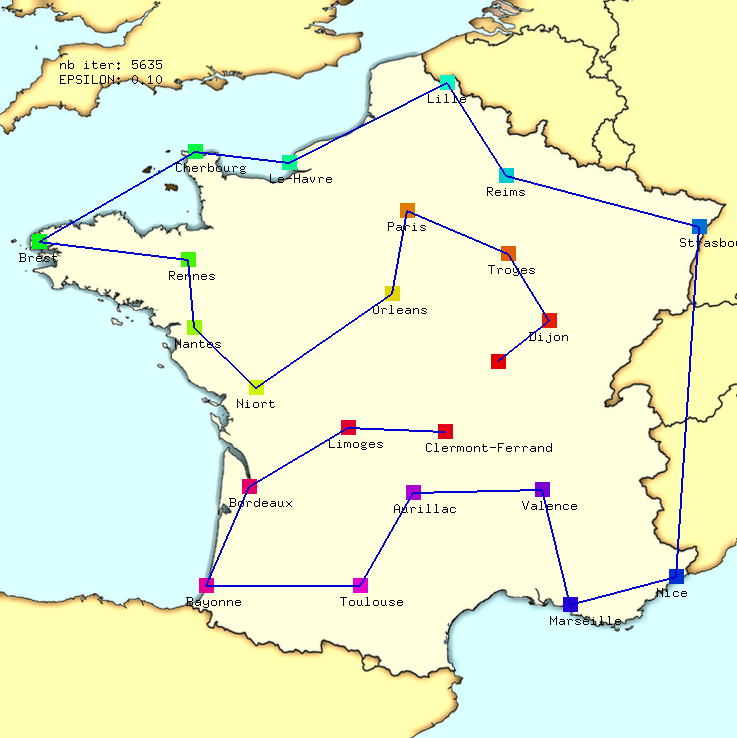
\includegraphics[width=25em]{tsp.png}
   \caption{Exemple de résultat du program}
\end{figure}

\section{Exercice 3}
\subsection{Questions préliminaires}
\subsubsection{ }
On peux utiliser une carte kohonen pour trouver les 16, 32 ou 256 meuilleurs
couleurs à utiliser pour l'image compressé, le réseau aura un vecteur d'entrée
de taille 3 (pour les composantes RGB), et la taille de neurones devra
correspondre aux nombre de couleurs dans l'image compressé. En plus on peux
avoir un topologie 2D de neurones (càd pour 16 couleurs une carte 4x4).
Pour l'apprentissage le donnée d'entrée c'est les pixels de l'image originale,
et un amélioration de ça pour les images de trés grande tailles, on peux sous-échantillonner
l'image a des blocs de pixels de taille fixe (4x4 par exemple) et on prend le
moyenne de ces pixels comme données d'entrée, cela servira a optimiser le
performance au niveau d'utilisation mémoire.\\

Pour le dernier étape aprés l'apprentissage on devra utiliser ces couleurs dans
l'image compressé, et pour faire ça, on regarder toutes les pixels de l'image
originale et on cherche de trouver le couleur (dans les poids de neurones) le
plus proche de ce pixel original, on peux definir la distance entre deux
couleur comme étant la norme (distance euclidienne) entre les deux vecteurs de
taille 3.
\begin{equation}
   dist(c1, c2) = \sqrt{(c1.R - c2.R)^2 + (c1.G - c2.G)^2 + (c1.B - c2.B)^2}
\end{equation}
\begin{figure}[H]
   \centering
   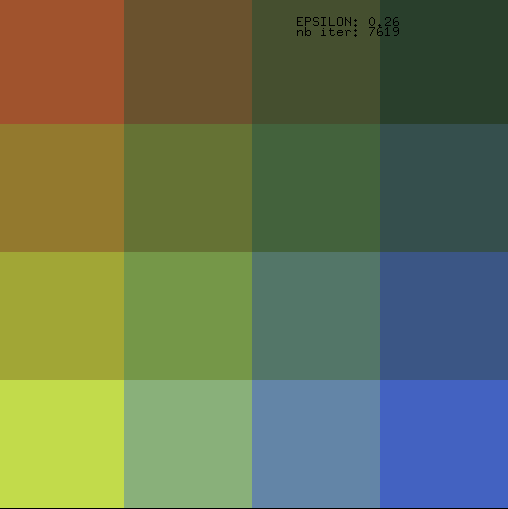
\includegraphics[width=25em]{cols.png}
   \caption{Exemple de 16 couleurs résultat sur l'image perroquet.ppm}
\end{figure}


\vspace{1mm}
\subsubsection{ }
Le nombre de bits pour un seul composant couleur (RGB): $\log_2{256} = 8$.\\
Pour un pixel RGB: $8 * 3 = 24$.\\
Le nombre de bits pour coder 16 couleur: $\log_2{16} = 4$.\\
Le facteur de gain de compression par rapport à l'originale: $24 / 4 = 6$.\\
Le facteur de gain de compression par rapport à un image NB: $8 / 4 = 2$.\\
Alors l'image compressé est 6 fois plus petit que l'originale et 2 fois plus
petit que l'image noir et blanc.

\subsection{Questions}
\subsubsection{ }
\begin{figure}[H]
   \centering
   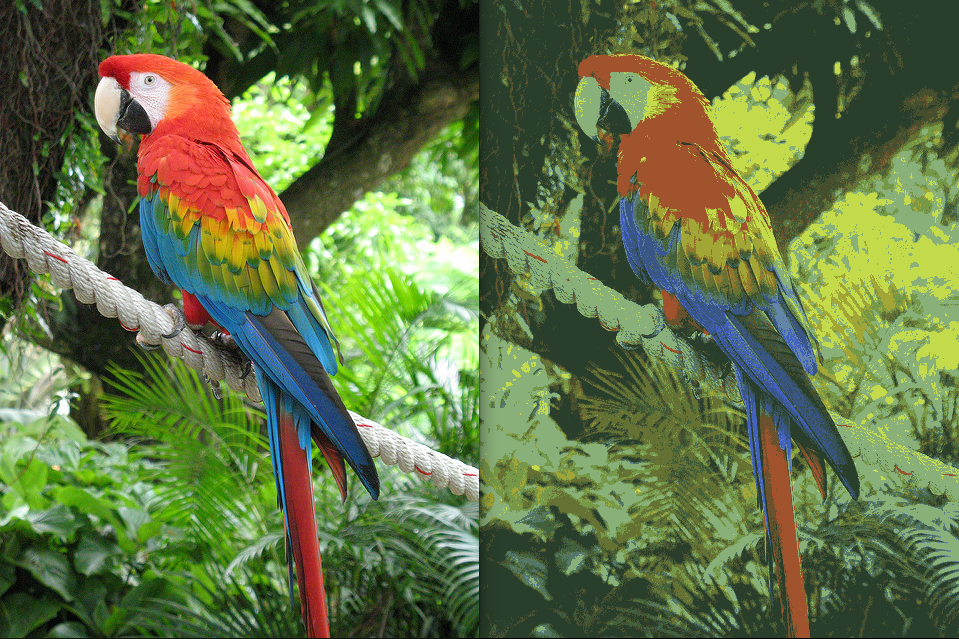
\includegraphics[width=25em]{comp.png}
   \caption{Compression avec 16 couleurs}
\end{figure}

\begin{figure}[H]
   \centering
   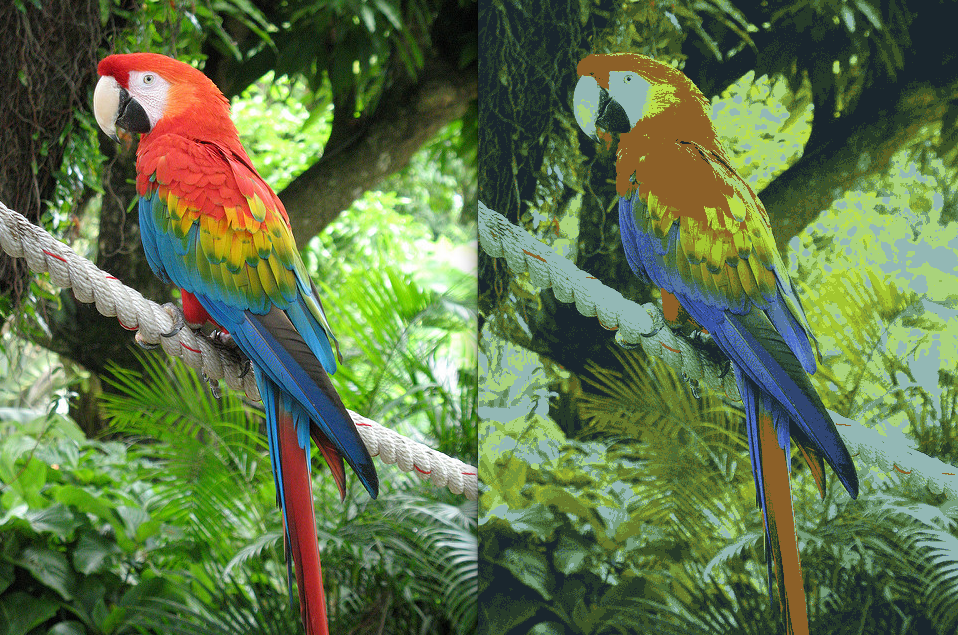
\includegraphics[width=25em]{comp32.png}
   \caption{Compression avec 32 couleurs}
\end{figure}

\begin{figure}[H]
   \centering
   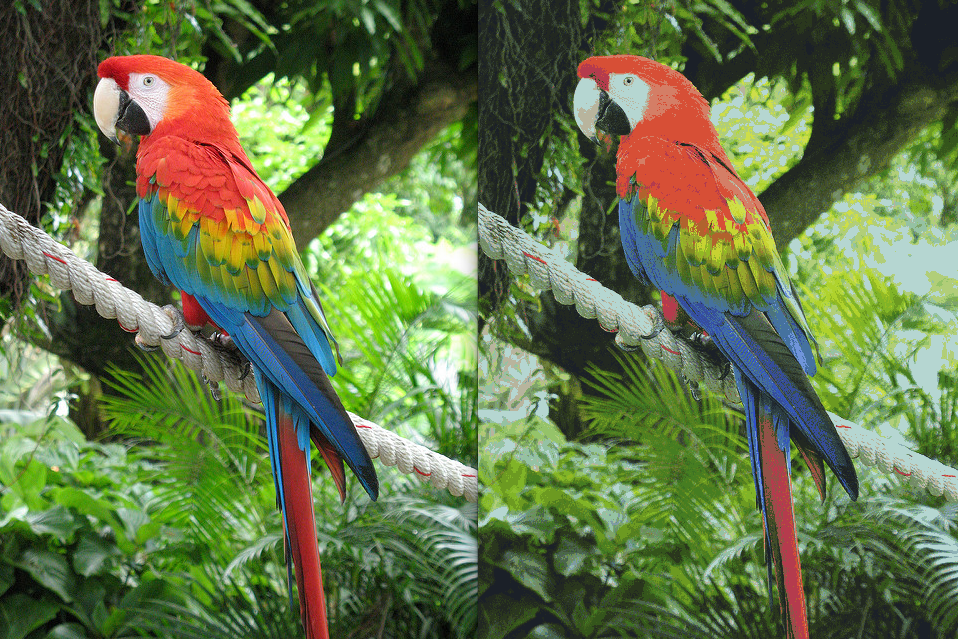
\includegraphics[width=25em]{comp256.png}
   \caption{Compression avec 256 couleurs}
\end{figure}

\subsubsection{ }
Le probléme c'est que les tailles de l'image compressé et l'originale
sont les mêmes. Pour régler ça, il faut utliser un format different pour le
stockage de l'image (à la place de .ppm), ce format doit exploiter le fait que
nous n'utilisons qu'un nombre de couleurs prédéfini pour notre image 



\end{document}

